\subsubsection{基于DoG算子的特征检测子(SIFT)}

\textbf{Lowe(2004)提出LoG近似等价于相邻尺度的高斯差分(DoG)}

高斯空间
\begin{equation*}
    L(x,y,\sigma) = G(x,y,\sigma) * I(x,y)
\end{equation*}

高斯差分(DoG)

\begin{flalign*}
    D(x,y,\sigma) &= (G(x,y,k\sigma) - G(x, y, \sigma)) * I(x,y)\\
    &= L(x,y,k\sigma) - L(x, y, \sigma)
\end{flalign*}

\textbf{DoG差分空间:} 

每个Octave的图像进行一次2倍的将采用,将采用得到的尺度$\sigma$为原来的两倍。

\begin{figure}[h]
\centering
\begin{minipage}[t]{0.48\textwidth}
\centering
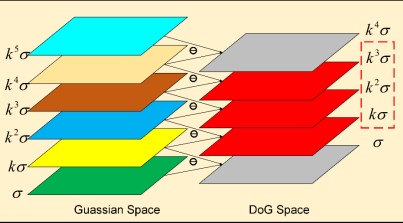
\includegraphics[width=6cm]{DoG差分Octave1.png}
\caption{Octave 1}
\end{minipage}
\begin{minipage}[t]{0.48\textwidth}
\centering
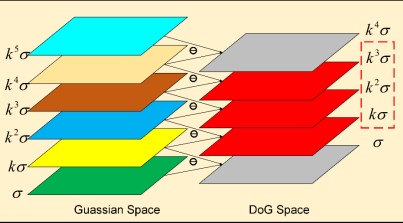
\includegraphics[width=6cm]{DoG差分Octave1.png}
\caption{Octave 2}
\end{minipage}
\begin{minipage}[t]{0.48\textwidth}
\centering
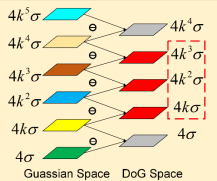
\includegraphics[width=6cm]{DoG差分Octave3.png}
\caption{Octave 3}
\end{minipage}
\end{figure}

阶数:$O = 3$

每阶的有效差分数:$S=3$  (有效差分数为去掉首尾的,图中DoG空间的红色部分)

每阶层数:$N=S+3$

这样设计的目的是保证每阶的DoG空间有效差分层最后一个的尺度正好等于下一阶的第一层尺度的一半。
这就使得DoG空间尺度上是连续、等间隔的。

\textbf{查找DoG空间离散极值点:} 

\begin{figure}[h]
    \centering
    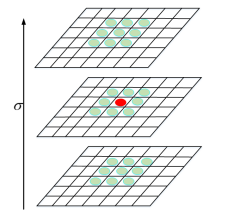
\includegraphics{DoG寻找极值点.png}
    \caption{DoG寻找极值点}
\end{figure}

在寻找极值点时,会比较上下两个尺度的图片中的除了自身以外的相邻的$4*4*3-1=47$个像素值。
当前像素值大于这相邻的其它47个像素值,则该点为极值点。

\textbf{通过泰勒展开近似查找亚像素DoG空间离散极值点:} 

利用二阶泰勒近似寻找极值点

\begin{flalign*}
\text{对$f(x_0)$进行泰勒二阶展开近似}\\ 
f(x) &\approx f(x_0) + \nabla f(x_0)^T(x-x_0) + \frac{1}{2}(x-x_0)^T\nabla^2f(x_0)(x-x_0) \\
\text{剔除常数项$f(x_0)$,并令$\delta x=x-x_0$得:}\\ 
f(\delta x) &= \nabla f(x_0)^T\delta x + \frac{1}{2}\delta x^T\nabla^2f(x_0)\delta x \\
\text{求一阶导,并令其为0:}\\ 
\frac{\partial f(\delta x)}{\partial \delta x} &= \nabla f^T(x_0) + \nabla^2f(x_0)\delta x = 0 \\
\text{整理上式得:}\\ 
\delta x &= -\nabla^2 f(x_0)^{-1} \nabla f^T(x_0)
\end{flalign*}

其中$\delta x$为在$x_0$点的近似极值点。